\chapter{Enhedstest}
I dette afsnit beskrives hvordan enhedstest af systemets enheder er udført. Enhedstesten bruges til at verificerer, at hver enkel del virker uafhængigt af andre enheder. 
Der testes primært basal funktionalitet af enhederne, og i nogle tilfælde undersøges hvorvidt krav fra kravspecifikationen opfyldes. I afsnittet testes blandt andet præcision af GPS og højdemåler.


\section{3G modul}

Enhedstest af 3G modulet foregår ved test af PUT og GET request, som er de metoder der er implementeret på dronen.

For udelukkende at have fokus på 3G modulet under enhedstesten, testes der ikke op imod den server som ellers anvendes til projektet. I stedet benyttes hjemmesiden requestb\footnote{requestb.in} , en hjemmeside der der tillader test af HTTP kommunikation. Ved at tilgå Requestb og starte en session tildeles en URL der kan bruges til test. Requestb indsamler information om alle HTTP request lavet til den tildelte URL. 

På figur \ref{fig:get_req} vises et GET request der sendes fra 3G modulet til en requestb.in server. Den første linje efter \textit{data:} fortæller om requestet er gennemført succesfuldt eller ej. Svaret \textit{200 ok} betyder at GET requestet er gået igennem og det ønskede data på korrekt vis er hentet. 

\vspace{0.3cm}

\begin{figure}[H]
\centering
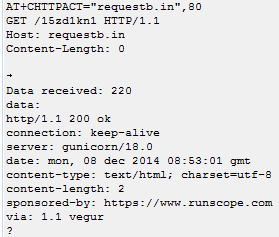
\includegraphics[width=0.5\textwidth]{Billeder/Test/get_requestbin.png}
\caption{GET Request}
\label{fig:get_req}
\end{figure}

\newpage

PUT request bruges til at sende data til eller opdatere information på server. 
På figur \ref{fig:putrequest_module} vises et PUT der sendes fra 3G modulet til requestb.in. De føreste seks linjer på figur \ref{fig:putrequest_module} viser requestet header med linje syv er requestet body. 

\begin{figure}[H]
\centering
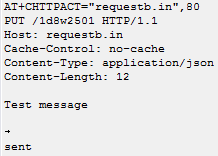
\includegraphics[width=0.5\textwidth]{Billeder/Test/putrequest_module.png}
\caption{PUT metode}
\label{fig:putrequest_module}
\end{figure}

\vspace{1cm}

På figur \ref{fig:put_req} vises det information der tilgængelig på server efter PUT requestet er fuldført. \textit{RAW BODY} viser det data der er modtaget og HEADERS indeholder parametrene for HTTP protokollen.

\begin{figure}[H]
\centering
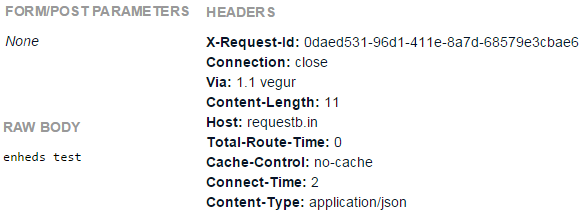
\includegraphics[width=0.8\textwidth]{Billeder/Test/put_request.png}
\caption{Information på server}
\label{fig:put_req}
\end{figure}



\newpage
\section{Afstandssensor}

I denne sektion beskrives hvordan ultralydssensoren HC-SR04 er testet for at fastslå hvor pålidelig den er. Testen er udført ved at lave gentagne målinger af afstand mellem ultralyds sensor og en væg. For hver deltest er der foretaget 100 målinger og maksimal værdi, minimal værdi og gennemsnit fundet. 

Ultralydssensoren bruges både til højdemåling og antikollison. Testen bruges til at kontrollere hvorvidt sensoren kan opfylde krav om nøjagtighed til højdemåling\footnote{Se ikke funktionelle krav i \textit{Kravspecifikation}}. 

Undervejs i testen ændres vinklen mellem ultralydssensor og væg, hvilket indirekte betyder afstande også ændres til væggen. I udgangspunkt skyder sensoren lyd ud i vandret retning og efterhånden ændres vinklen. Det formodes at sensoren fungerer bedst når der er en 90 graders vinkel mellem sensor og væg. 

På figur \ref{fig:ultra_testopstilling} vises en skitse af den anvendte testopstilling og tabellen nederst på siden viser resultater af den udførte test.

\begin{figure}[H]
\centering
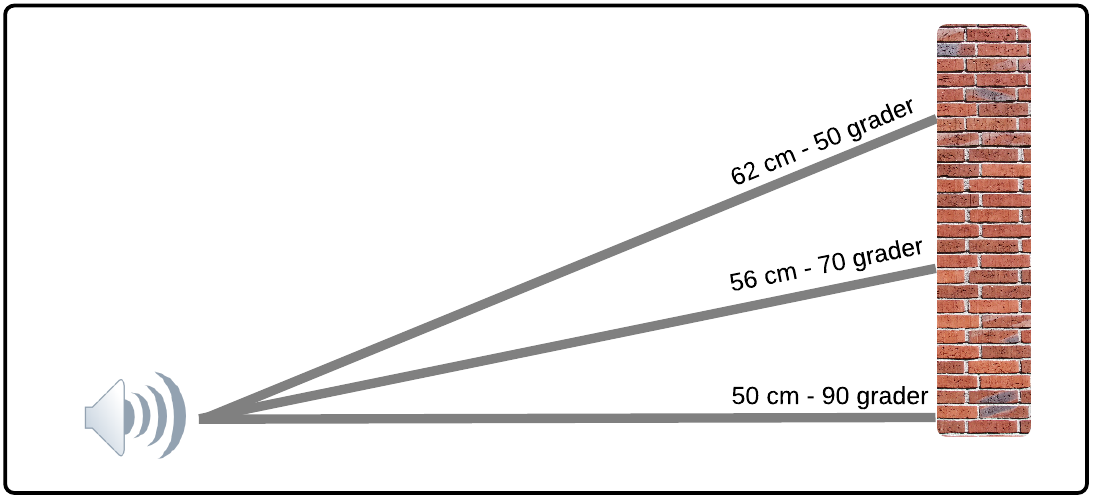
\includegraphics[width=1\textwidth]{Billeder/Test/ultrasound.png}
\caption{Skitse af testopstilling}
\label{fig:ultra_testopstilling}
\end{figure}

\vspace{0.5cm}

\begin{table}[H]
\begin{tabular}{| p{2.5cm}| p{2.5cm}| p{2.5cm}| p{2.5cm}| p{2.5cm}|}
\hline
\textbf{Vinkel} & \textbf{Afstand} & \textbf{Maks måling} & \textbf{Min måling}  & \textbf{Middel værdi} \\ \hline
0 & 50 cm & 49.0 cm & 48.0 cm  & 48.02 cm \\ \hline
20 & 56 cm & 49.0 cm & 49.0 cm  & 49.0 cm \\ \hline
40 & 62 cm & 50.0 cm & 51.0 cm  & 50.0 cm \\ \hline

\end{tabular}
\caption{Test ultralydssensor}
\label{tab:Ultralyds_test}
\end{table}




\newpage
\section{GPS}

Selvom GPSen sidder på 3G/GPS modulet kan det testes for sig selv. 

For at finde den eksakte GPS position fra GPS modulet, testes modulet i forskellige omgivelser. Som kontrol findes koordinaterne for den aktuelle position. Ud fra de fundne koordinater beregnes en afstand i meter, denne afstand fortæller lidt om afvigelsen af GPS modulet. I kravene er der defineret hvor stor en afvigelse GPS modulet må have. Denne afvigelse skal overholdes under tests, men da den aktuelle position har en afvigelse, vil afgivelsen i meter være påvirket. Denne påvirking vil føre til at afvigelsen i meter kan være større end de tilladte 2.5 meter som der er defineret i kravene.
Det har ikke været muligt at teste GPS modulet indendøre, da der ikke var GPS signal tilgængeligt. 

\begin{table}[H]
\begin{tabular}{| p{4cm}| p{4cm}| p{3cm}|}
\hline
GPS moduls koordinater & Aktuelle position & Afvigelse i meter\\\hline
Latitude:10.191518 \newline Longitude: 56.171863 & Latitude: 10.191560 \newline Longitude: 56.171896 & 4 meter\\\hline
Latitude: \newline Longitude & Latitude: \newline Longitude & \\\hline
Latitude: \newline Longitude & Latitude: \newline Longitude & \\\hline

\end{tabular}
\caption{GPS modul}
\label{tab:GPS_modul}
\end{table}



\newpage 
\section{PWM opsætning}

Testen bruges til at fastslå hvorvidt det PWM signal, der genereres af main controller, udsendes med korrekt frekvens og pulsbredde. Testen foregår ved at ændre værdien af compare-registeret\footnote{Se implementation view i \textit{Systemarkitektur og Design}} . Ændringer i compare registerets værdi bør medføre ændringer af pulsbredde i det PWM signal der udsendes fra main controller. 

Indledningsvis indstilles compare-registeret med værdi på 16000, derefter ændres værdien til 24000 og til sidst sættes compare-registerets værdi til 32000. Ved brug af oscilloskop kontrolleres om PWM signal har den korrekte pulsbredde. 

Nedenfor ses en tabel der viser hvordan testen forløb. Efter tabellen vises oscilloskop billeder taget under testen. 

\vspace{0.50cm}

\begin{table}[H]
	\centering
		\begin{tabular}{|c|c|c|c|}
			\hline
			Værdi compare reg. & Frekvens & Forventet pulsbredde & Faktisk pulsbredde \\ \hline
			16000 & 245 Hz & 1.00 ms & 1.00 ms \\ \hline			
			24000 & 245 Hz & 1.50 ms & 1.50 ms \\ \hline
			32000 & 245 Hz & 2.00 ms & 2.00 ms \\ \hline
		\end{tabular}
	\caption{Test resultat}
\end{table}

\vspace{0.50cm}

Figur \ref{fig:PWM_1} vises PWM signal hvor compare register har værdi på 16000. 

\begin{figure}[H]
\centering
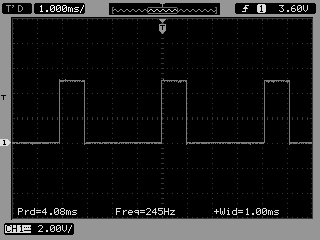
\includegraphics[width=0.7\textwidth]{Billeder/Test/PWM_16000.png}
\vspace{-0.0cm}
\caption{PWM signal - Compare register 16000}
\label{fig:PWM_1}
\end{figure}

\newpage

Figur \ref{fig:PWM_2} vises PWM signal hvor compare register har værdi på 24000. 
\begin{figure}[H]
\centering
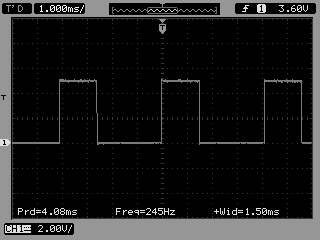
\includegraphics[width=0.7\textwidth]{Billeder/Test/PWM_24000.png}

\caption{PWM signal - Compare register 24000}
\label{fig:PWM_2}
\end{figure}

\vspace{0.5cm}

Figur \ref{fig:PWM_3} vises PWM signal hvor compare register har værdi på 32000. 
\begin{figure}[H]
\centering
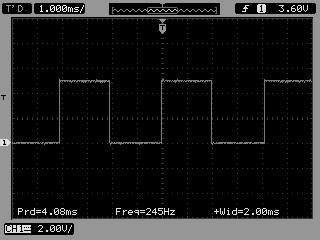
\includegraphics[width=0.7\textwidth]{Billeder/Test/PWM_32000.png}
\vspace{-0.0cm}
\caption{PWM signal - Compare register 32000}
\label{fig:PWM_3}
\end{figure}

%\newpage
%\section{Enhedstest software}
Til test af softwaren til systemet er enhedstests benyttet. Enhedstest er den test metode hvor softwaren deles op i mindst mulige dele og tests helt isolerede fra resten af systemet. Under enhedstest sikres at hver enhed i systemet fungere efter hensigten. Enhedstest bliver udarbejdet samtidig med produktions koden  bliver udviklet, på den måde bliver de fleste fejl i systemet fanget, mens systemet er under udvikling. Dvs fejl i systemet bliver opdaget samtidig med at systemet er under udvikling, hvilket mindsker fejlens omfang og omkostninger for at rette fejlen.

På figur \ref{fig:test_forlob} ses mængende af fejl i div testforløb og fokus opdelningen.
\begin{figure}[H]
	\centering
	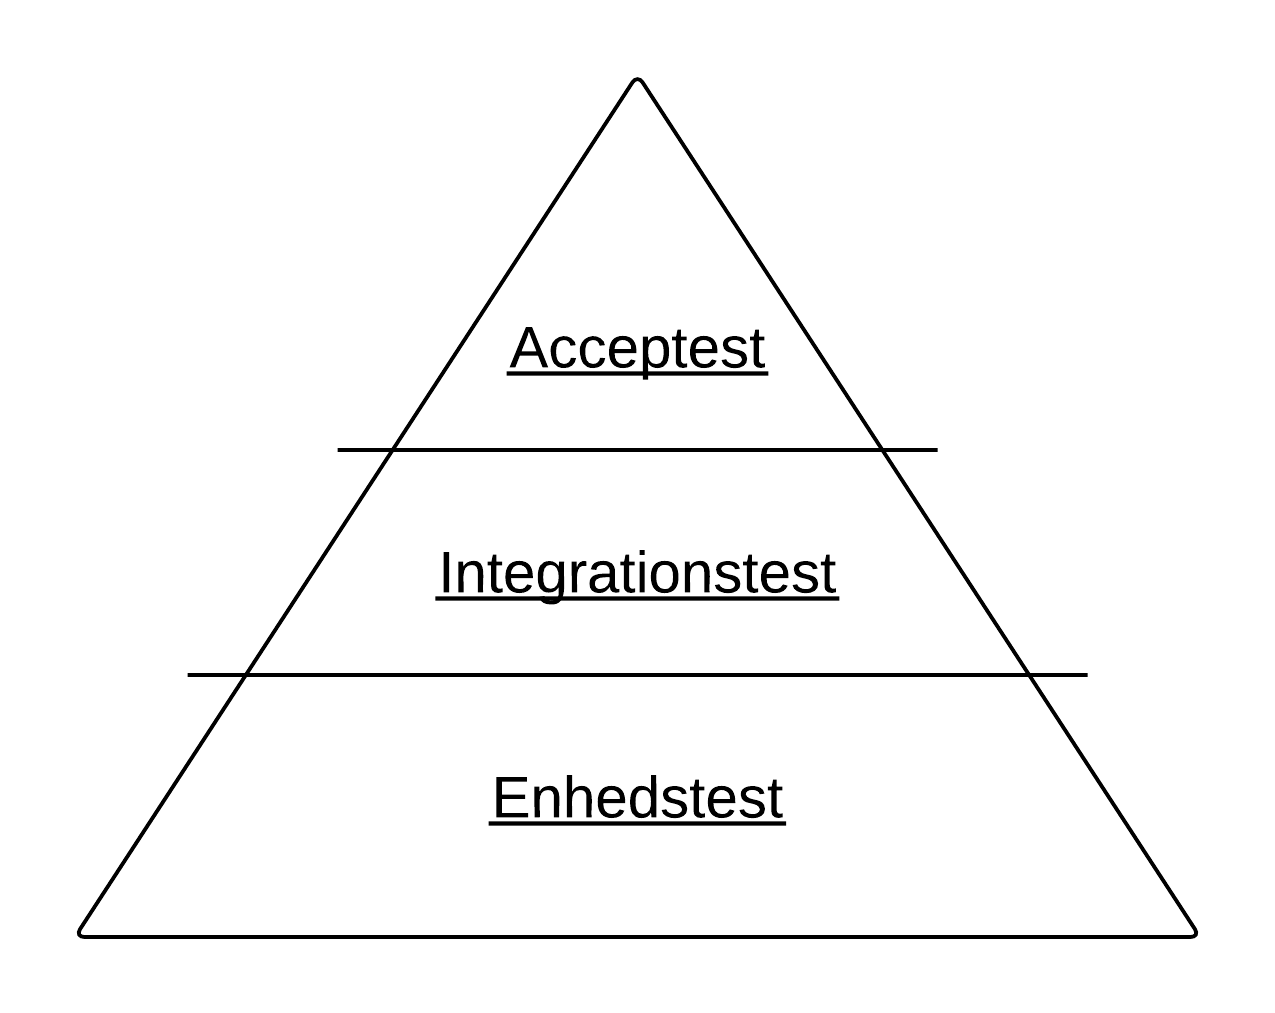
\includegraphics[width=0.6\textwidth]{Billeder/Test/forlob.png}
	\caption{Mængden af fejl}
	\label{fig:test_forlob}
\end{figure}

\subsection{Test opbygning}
Enhedstestene er opbygget efter AAA-modellen\footnote{http://c2.com/cgi/wiki?ArrangeActAssert}.\\ 
Arrange: \\
Her opsættes input til testen, eller evt afhængigheder håndteres. \\
Act: \\
Her bliver det ønskede kode stimuleret. \\
Assert: \\
Her forventes et bestemt output og testen afgøres om den er succesfuld eller ej.

\newpage
På  figur \ref{fig:aaa} ses et eksempel på AAA modellen. I testen bliver der testet for om den korrekte metode bliver kaldt når bruger prøver at logge in på webapplikationen. 

\begin{figure}[H]
	\centering
	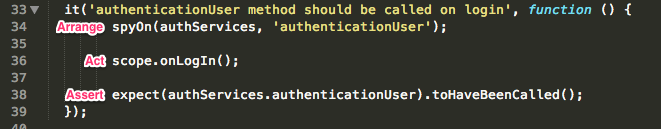
\includegraphics[width=0.6\textwidth]{Billeder/Test/aaa.png}
	\caption{AAA eksempel}
	\label{fig:aaa}
\end{figure}

\newpage
\input{Kapitler/Test/Webapplikation}
